%%=============================================================================
%% Conclusie
%%=============================================================================

\chapter{Conclusie}
\label{ch:conclusie}

% TODO: Trek een duidelijke conclusie, in de vorm van een antwoord op de
% onderzoeksvra(a)g(en). Wat was jouw bijdrage aan het onderzoeksdomein en
% hoe biedt dit meerwaarde aan het vakgebied/doelgroep? 
% Reflecteer kritisch over het resultaat. In Engelse teksten wordt deze sectie
% ``Discussion'' genoemd. Had je deze uitkomst verwacht? Zijn er zaken die nog
% niet duidelijk zijn?
% Heeft het onderzoek geleid tot nieuwe vragen die uitnodigen tot verder 
%onderzoek?

In het vorig hoofdstuk werden de gekozen module bundlers op de proef gesteld aan de hand van drie open-source projecten en een van nul te beginnen. De verschillende stappen om ze werkende te krijgen werden overlopen, bij de een waren dat er al meer dan de ander. In dit hoofdstuk wordt gekeken naar de gemeten en waargenomen resultaten, objectief en subjectief, om tot een conclusie te komen.

\section{Nieuw project}

Al de module bundlers hebben niet gezweet bij het opzetten van een nieuw project, wat maar normaal is. Voor Webpack is er gebruik gemaakt van een framework, CRA, omdat het configuratie werk anders te veel zou zijn. Ookal is het een nieuw project en dus relatief klein, toch kunnen we al verschillen waarnemen tussen de vier kandidaten. 

Op onderstaande figuur zien we al een trend verschijnen die doorheen deze conclusie zal gelden: Webpack is aanzienlijk trager dan de competitie, ondanks dat Snowpack niet bundelt, is het toch even traag of trager dan Parcel. Die laatste zijn Rust compiler, zie literatuurstudie, zal zijn vruchten afwerpen. De drie balkjes die ontbreken bij Vite en het ene bij Parcel zijn geen fout: ze waren gewoon sneller dan een volledige seconde. 

\begin{figure}[h]
    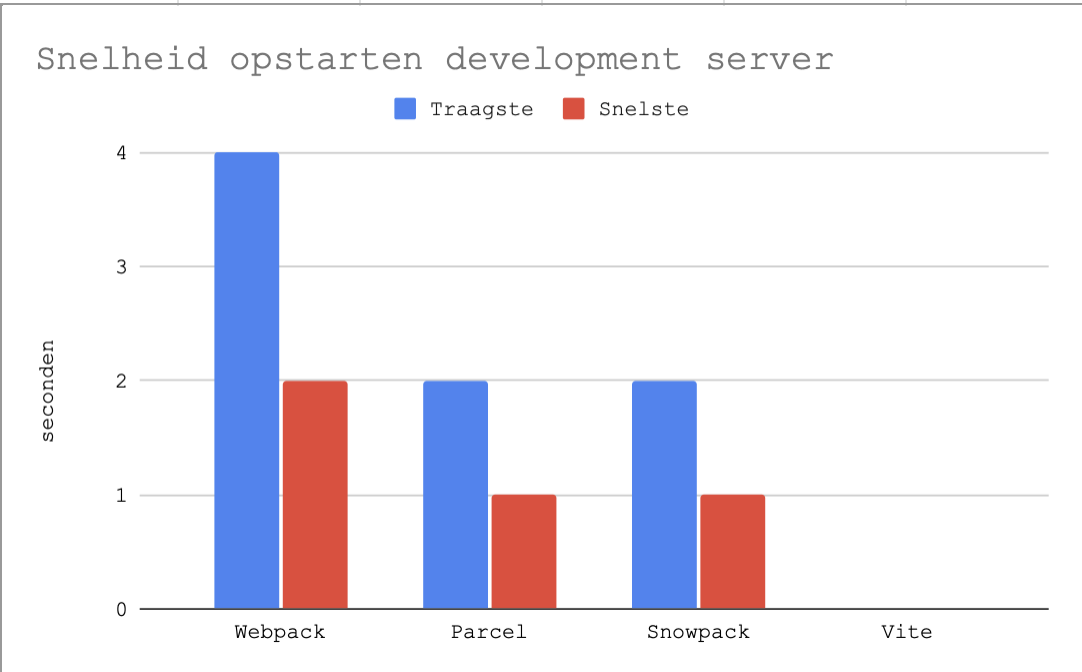
\includegraphics[scale=0.6]{conslusieNieuwDev}
        \centering
        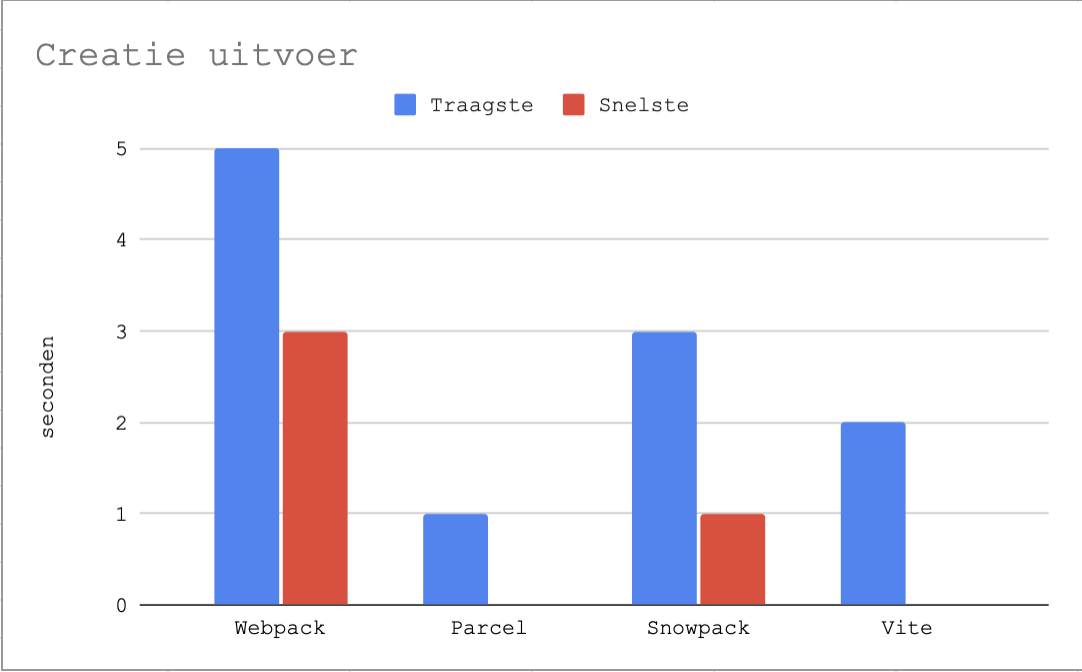
\includegraphics[scale=0.6]{conclusieNieuwUitvoer}
        \centering
        \caption{Resulaten nieuw project}
    \end{figure}


De developer experience was voor al de build tools zo goed als hetzelfde bij het opzetten van dit nieuw project. De conclusie kunnen we daarop dus niet baseren. Maar de data hierboven is duidelijk genoeg: bij het opzetten van een project is Vite de beste optie. Het gebruikt het beste van beide werelden: ongebundelde code in development en gebundelde code in productie. De andere opties hebben niet direct een afknapper, maar de snelheid van Vite valt niet te negeren.

\section{Bestaand project}
Een bestaand project omvormen is het heel andere koek gepaard met andere overwegingen. In de methodologie is getracht projecten te kiezen met zoveel mogelijk uiteenlopende technologieën. Natuurlijk is lang niet alles aan bod gekomen. Een project kan bestaan uit talloze combinaties van verschillende, soms niche technologieën, packages of zelf geschreven bibliotheken. Wat in dit onderzoek geconcludeerd zal worden, is een overweging gebaseerd op de projecten die hier aan bod gekomen zijn. Het kan zijn dat voor een ander project, die keuze minder gemakkelijk of zelfs uitgesloten is door welke factor dan ook. Dat terzijde, de conclusie zal in het algemeen voor de meesten gelden aangezien veel voorkomende use-cases aan bod kwamen. Onderstaande resultaten zouden hoogstwaarschijnlijk nog kunnen bijgeschaafd worden door van elke build tool de configuratie te optimaliseren per project. Dit echter is niet het punt van deze studie. Welke build tool is in het algemeen de beste keuze, zonder uren de configuratie bij te schaven?

Op onderstaande figuur is te zien dat elke geteste build tool het beter doet dan Webpack en het verschil is vaak niet klein. Hoewel Snowpack ook aanzienlijk sneller maar aangezien uit de methodologie is gebleken dat de developer experience ver van optimaal is, zeker in vergelijking met de andere opties, kijk je beter elders bij het kiezen van een nieuwe build tool. Parcel en Vite daarentegen doen het heel goed op vlak van developer experience en snelheid. Parcel levert gebundelde code af, ook in development. Dit kan een voor- of nadeel zijn, afhangend hoe het bekeken wordt. Uit het vorig hoofdstuk blijkt dat Vite geen CommonJS ondersteunt, Parcel wel. Hoewel Parcel in sommige scenario’s net iets sneller weet te zijn dan Vite, wint die laatste toch in de meeste gevallen. Merk op dat ook bij de tweede grafiek, het balkje bij Vite ontbreekt. Dit is weer geen fout: Vite slaagt erin om zijn development server gemiddeld in sneller dan een seconde op te starten. Dat is indrukwekkend, zeker als dit naast de resultaten van de competitie gelegd wordt. 

\begin{figure}[h]
    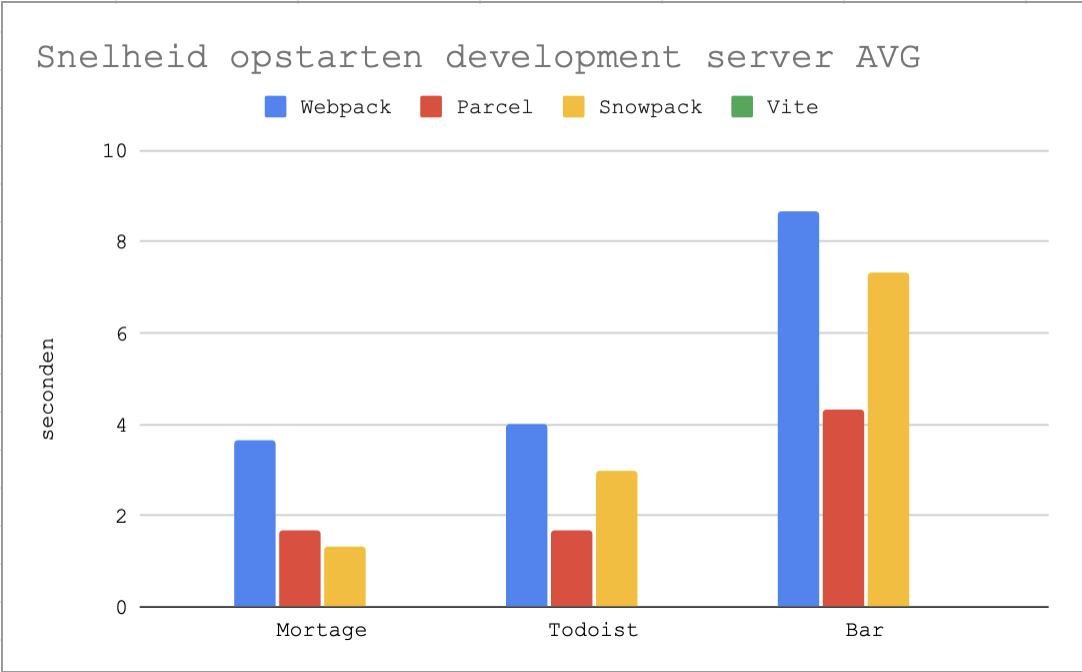
\includegraphics[scale=0.6]{conclusieBestaandDev}
        \centering
        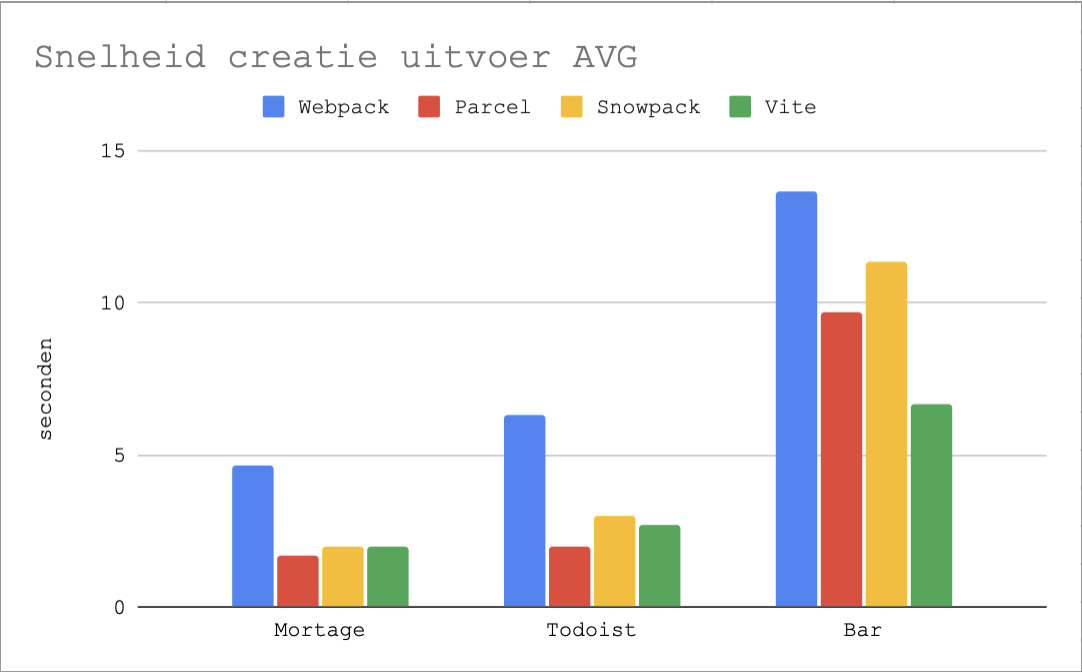
\includegraphics[scale=0.6]{conclusieBestaandUitvoer}
        \centering
        \caption{Resulaten bestaand project}
    \end{figure}

    De opzet van deze proef, of Webpack nog steeds mag gezien worden als de koning der module bundlers, kan dus beantwoord worden met een duidelijke ‘nee’. Zelf binnen zijn eigen categorie van gebundelde code, blijkt Parcel, in de meeste gevallen, een betere optie te zijn. 